\section{Entropia}
\subsection{Definição de entropia}
\begin{frame}%[allowframebreaks]
  \frametitle{Entropia}
  \begin{definition}[Entropia]\label{def-entropia}
  Dada uma variável aleatória $X$ sob um alfabeto de tamanho finito $\mathcal{X}$, a \textbf{entropia}
  da variável aleatória é dada por
  \begin{eqnarray}
  H(X) &\triangleq& E_p \log \frac{1}{p(X)} = E \log \frac{1}{p(X)} \\
        &=& \sum_{x \in \mathcal{X}} p(x) \log \frac{1}{p(x)} = - \sum_x p(x) \log p(x)
  \end{eqnarray}
  \end{definition}
  A unidade de entropia é `bits', já que utilizamos o logaritmo na base $2$ (unidade `nats' se 
  utilizar a base $e$).
\end{frame}
\note{  
  \begin{itemize}
  \item Entropia mede a grau de incerteza associado a uma distribuição.
  \item Entropia mede a desordem ou o espalhamento de uma distribuição.
  \item Entropia mede a `escolha' que a fonte tem na escolha de símbolos de acordo com uma densidade 
        (maior entropia implica em mais escolha).
  \item Vamos utilizar a seguinte convenção: $0 \log 0 = 0$.
  \end{itemize}
}

\begin{frame}%[allowframebreaks]
  \frametitle{Entropia}
  Se uma v.a. $X \sim p(x)$, então o valor esperado de uma função desta v.a., $g(X)$, é dada por
  \begin{equation}
  E[g(X)] = \sum_{x \in \mathcal{X}} p(x) g(x) .
  \end{equation}

  A entropia de $X$ pode ser interpretada como o valor esperado da v.a. $\log \frac{1}{p(X)}$,
  onde $X$ é descrita pela função massa de probabilidade $p(x)$.
  \begin{equation}
  H(X) = E \left[ \log \frac{1}{p(X)} \right] .
  \end{equation}
\end{frame}
\note{
  \begin{itemize}
  \item Entropia é uma medida da real `incerteza' média, o que é uma medida sobre toda a distribuição.
  \item Entropia mede o grau de incerteza médio ou esperado do resultado de uma distribuição de probabilidade.
  \item É uma medida de desordem ou espalhamento. Distribuições com alta entropia devem ser planas, mais
  uniformes, enquanto distribuições com baixa entropia devem possuir poucas modas (unimodal, bimodal).
  \end{itemize}
}
\note{
  \begin{figure}[h!]
  \centering
  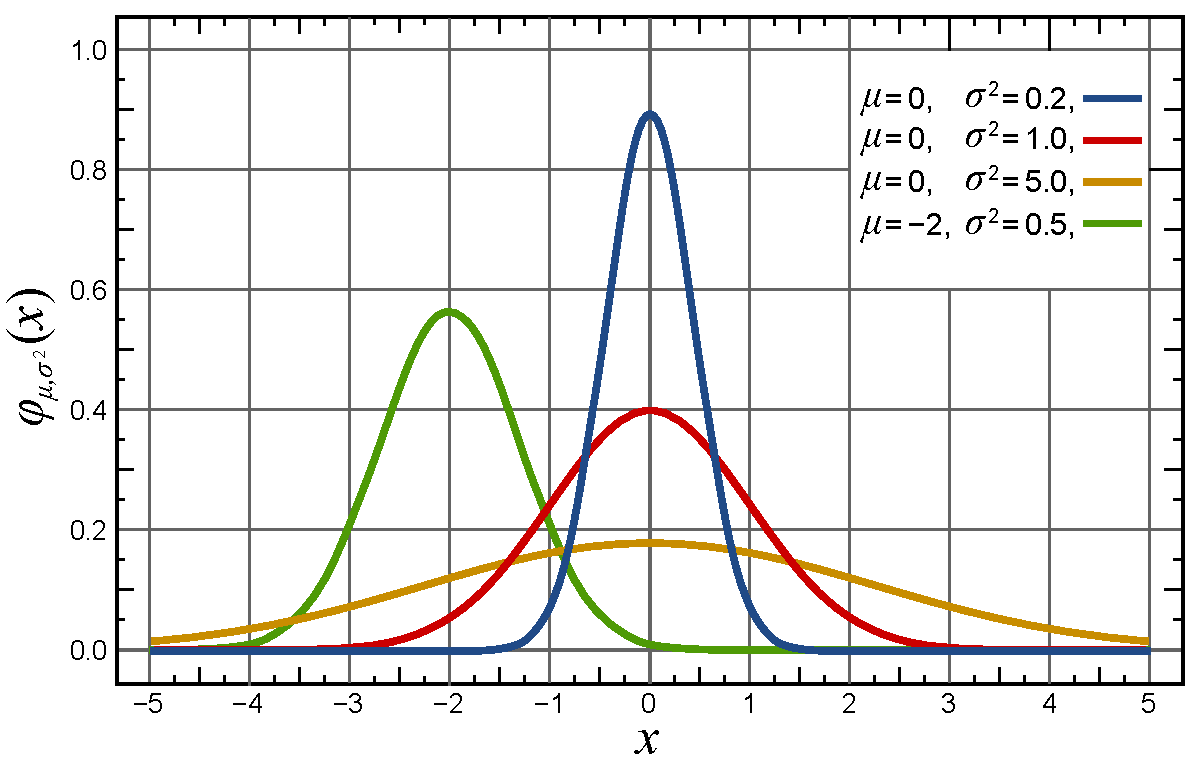
\includegraphics[width=0.4\textwidth]{images/normal_distribution.pdf}
  %\caption{.}
  \label{fig:normal_distribution}
  \end{figure}

  \begin{itemize}
  \item mais concentrado: menor entropia
  \item mais espalhado: maior entropia
  \item os valores em $x$ não importam, 
  apenas os valores das probabilidades associadas $p(x)$ importam no cálculo da entropia
  \end{itemize}
}

\begin{frame}[allowframebreaks]
  \frametitle{Escolha, Incerteza e Entropia}
  Suponha um conjunto de eventos cujas probabilidades de ocorrências sejam dadas
  por $p_1, p_2, \ldots, p_n$. É possível encontrar uma medida de quanta `escolha' 
  está envolvida na seleção de um evento ou quão incertos estamos da saída?

  Para tal medida $H(p_1, p_2, \ldots, p_n)$, é razoável requerermos as seguintes propriedades:
  \begin{enumerate}
  \item $H$ deve ser contínuo em $p_i$;
  \item Se todos os $p_i$ são iguais, $p_i=\frac{1}{n}$, então $H$ deve ser uma função
  monotonicamente crescente de $n$ (quando temos eventos equiprováveis, teremos mais incerteza
  quão maior for o número de eventos possíveis);
  \item Se for possível quebrar uma escolha em uma sequência de escolhas sucessivas,
  a medida $H$ original deve ser a soma ponderada dos valores individuais das medidas
  $H_i$ após a quebra.
  
     \begin{figure}[h!]
     \centering
     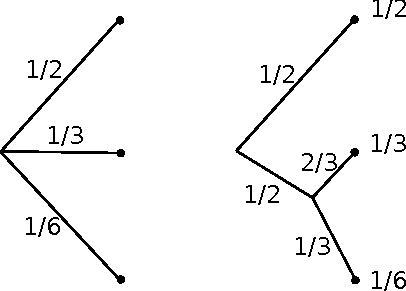
\includegraphics[width=0.3\textwidth]{images/entr-quebra.pdf}
     %\caption{Df.}
     \label{fig:entr-quebra}
     \end{figure}

  \begin{equation}
  H(\frac{1}{2},\frac{1}{3},\frac{1}{6}) = H(\frac{1}{2},\frac{1}{2}) + \frac{1}{2} H(\frac{2}{3},\frac{1}{3})
  \end{equation}
  \end{enumerate}

  A única função $H$ que satisfaz às suposições acima é da forma \cite{shannon1948}: 
  \begin{equation}\label{eq-K-entropia}
  H = - K \sum_{i=1}^{k} p(i) \log p(i) \textmd{ ,}
  \end{equation} 
  onde $K$ é uma constante positiva. 
\end{frame}




\subsection{Demonstração da equação da entropia}
\begin{frame}[allowframebreaks]
  \frametitle{Demonstração da \Cref{eq-K-entropia}}

  Nesta secção iremos apresentar a demonstração de $H=-\sum p_i \log p_i$ 
  (conforme Apêndice 2 de \citet{shannon1948}).

  Vamos definir
  \begin{equation}
  A(n) = H\left( \frac{1}{n}, \frac{1}{n}, \ldots, \frac{1}{n} \right) .
  \end{equation}

  Desejamos que uma escolha dentre $s^m$ opções igualmente prováveis possa ser decomposta como uma sequência de $m$ escolhas
  que se subdividem em $s$ possibilidades igualmente prováveis.

  \begin{figure}[h!]
  \centering
  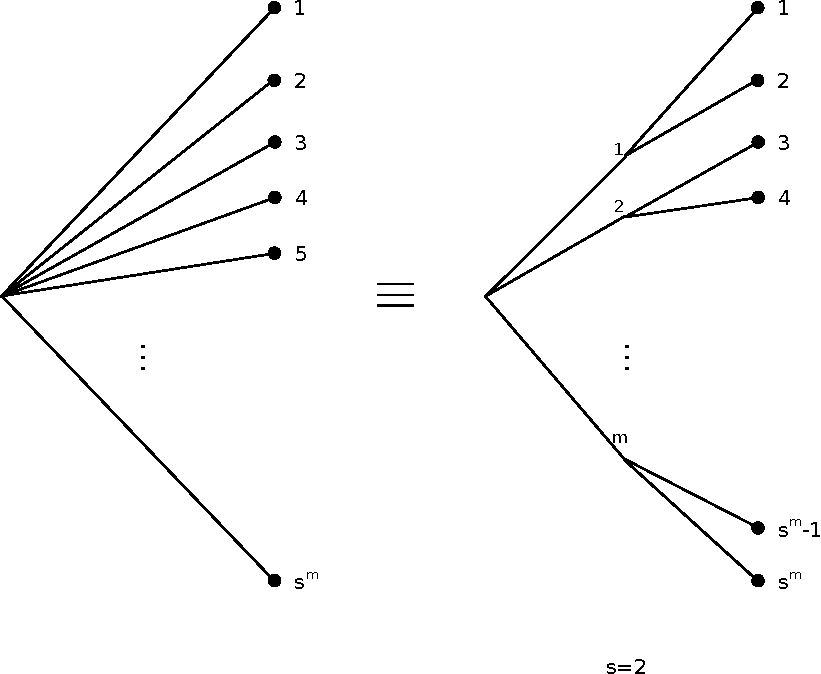
\includegraphics[width=0.5\textwidth]{images/choices.pdf}
  \caption{Exemplo de equivalência para $s=2$.}
  \label{fig:choiceseqv}
  \end{figure}

  Teremos então que
  \begin{equation}
  A(s^m) = m A(s) .
  \end{equation}
  Da mesma forma, para $t$ e $n$, teremos $A(t^n) = n A(t)$.
  Podemos tomar $n$ arbitrariamente grande e encontrar $m$ que satisfaça
  \begin{equation}
  s^m \leq t^n \leq s^{(m+1)} .
  \end{equation}
  Tomando o logaritmo\footnote{Logaritmo é uma função monótona crescente.} da expressão acima e dividindo 
  por $n \log s$ todos os termos\footnote{$n \log s$ é positivo para $n \geq 0$ e $s \geq 1$.}, teremos
  \begin{equation}
  \frac{m}{n} \leq \frac{\log t}{\log s} \leq \frac{m}{n} + \frac{1}{n} ,
  \end{equation}
  o que é equivalente a 
  \begin{equation}
  \left\vert \frac{m}{n} - \frac{\log t}{\log s} \right\vert < \epsilon ,
  \end{equation}
  onde $\epsilon$ é arbitrariamente pequeno, já que $n$ é arbitrariamente grande.

  Usando agora a propriedade desejada de monotonicidade de $A(n)$, teremos
  \begin{align}
  A(s^m) &\leq A(t^n) &\leq A(s^{(m+1)}) \\
  mA(s) &\leq nA(t) &\leq (m+1)A(s)
  \end{align}

  Dividindo a expressão acima por $nA(s)$, teremos
  \begin{equation}
  \frac{m}{n} \leq \frac{A(t)}{A(s)} \leq \frac{m}{n} + \frac{1}{n} ,
  \end{equation}
  ou, de forma equivalente,
  \begin{equation}
  \left\vert \frac{m}{n} - \frac{A(t)}{A(s)} \right\vert < \epsilon ,
  \end{equation}
  e assim, como as duas frações ($\nicefrac{\log t}{\log s}$ e $\nicefrac{A(t)}{A(s)}$) estão $\epsilon$ próximas
  de $\nicefrac{m}{n}$, podemos concluir que
  \begin{equation}
  \left\vert \frac{A(t)}{A(s)} - \frac{\log t}{\log s} \right\vert < 2\epsilon .
  \end{equation}
  Como $\epsilon$ é arbitrariamente pequeno, no limite teremos
  \begin{eqnarray}
  \frac{A(t)}{A(s)} &=& \frac{\log t}{\log s} \\
  A(t) &=& \frac{A(s)}{\log s} \log t = K \log t ,
  \end{eqnarray}
  onde $K$ deve ser positivo, de forma que $A(n)$ seja monótona crescente.

  Suponha uma escolha com $n$ possibilidades em que as probabilidades são comensuráveis,
  $p_i = \nicefrac{n_i}{\sum n_i}$, onde $n_i$ são inteiros. De forma equivalente,
  uma escolha entre $\sum n_i$ opções pode ser expressa como uma escolha dentre $n$ opções
  com probabilidades $p_1, \ldots, p_n$, e para uma $i$-ésima dada escolha, realizar uma
  nova escolha dentre $n_i$ opções igualmente prováveis. Teremos então:
  \begin{eqnarray}
  \overbrace{ K \log \left( \sum n_i \right) }^{A\left( \sum n_i \right)} &=& H(p_1, \ldots, p_n) + \overbrace{ K \log n_i }^{A(n_i)}\\
  K \underbrace{\left( \sum p_i \right)}_{=1} \log \left( \sum n_i \right) &=& H(p_1, \ldots, p_n) + K \underbrace{\left( \sum p_i \right)}_{=1} \log n_i .
  \end{eqnarray}  
  E assim,
  \begin{eqnarray}
  H(p_1, \ldots, p_n) &=& K\left[ \left( \sum p_i \right) \log \left( \sum n_i \right) - \left( \sum p_i \right) \log n_i \right] \\
        &=& -K \sum p_i \log \frac{n_i}{\sum n_i} = -K \sum p_i \log p_i . \qed
  \end{eqnarray} 
\end{frame}


